\documentclass[12pt,english,nohyper]{tufte-handout}
\usepackage[T1]{fontenc}
\usepackage[utf8]{inputenc}
\usepackage{longtable}
\usepackage{wrapfig}
\usepackage{hyperref}
\usepackage{graphicx}
\usepackage[space]{grffile}
\usepackage{geometry}
\usepackage{pgffor}
%\usepackage{caption}
\usepackage{calc}
\usepackage{enumitem}
\usepackage{microtype}
%\usepackage{floatrow} % test for caption below
\usepackage{tabularx}
%\usepackage[capposition=bottom]{floatrow}

\begin{document}



\centerline{\Large\bf Statistics 101 Homework Short Report for Topic 01 CD}
\vspace{1cm}

\begin{marginfigure}
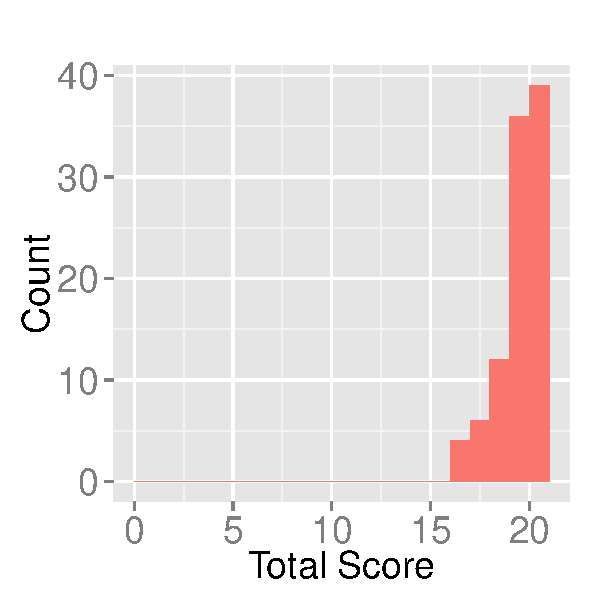
\includegraphics[width=0.98\linewidth]{Topic01_CD_score}
\caption{\label{mar:hist}Histogram of scores. Blue data represent scores less than 80 percent.}
\end{marginfigure}

% latex table generated in R 3.1.3 by xtable 1.7-4 package
% Wed Sep  9 19:34:42 2015
\begin{longtable}{llllllll}
  \hline
Mean & Std.dev &   & Min & Q1 & Median & Q3 & Max \\ 
  \hline
19.03 & 1.07 &  & 16.00 & 19.00 & 19.00 & 20.00 & 20.00 \\ 
  (95\%) & (5.4\%) &  & (80\%) & (95\%) & (95\%) & (100\%) & (100\%) \\ 
   \hline
\hline
\caption{Summary statistics of the scores} 
\label{tab:summary}
\end{longtable}
















